\documentclass[12pt,a4paper]{report}
\usepackage[utf8]{inputenc}
\usepackage[top=2.0cm, bottom=2.5cm, left=2.0cm, right=2.0cm, footskip=1.0cm]{geometry}
\usepackage{graphicx}
\usepackage{amsmath}
\usepackage{amssymb}
\usepackage{setspace}
\usepackage{tikz}
\usepackage{eso-pic}
\usepackage{fancyhdr}
\usepackage{listings}
\usepackage{xcolor}
\usepackage{booktabs}
\usepackage{array}
\usepackage{longtable}
\usepackage{caption}
\usepackage{tocbibind}
\usepackage{mathptmx} % Times New Roman style font
\usepackage[hidelinks]{hyperref}


% Document settings
\onehalfspacing
\definecolor{codegreen}{rgb}{0,0.6,0}
\definecolor{codegray}{rgb}{0.5,0.5,0.5}
\definecolor{codepurple}{rgb}{0.58,0,0.82}
\definecolor{backcolour}{rgb}{0.95,0.95,0.92}

% Listings setup
\lstdefinestyle{mystyle}{
    backgroundcolor=\color{backcolour},   
    commentstyle=\color{codegreen},
    keywordstyle=\color{magenta},
    numberstyle=\tiny\color{codegray},
    stringstyle=\color{codepurple},
    basicstyle=\ttfamily\footnotesize,
    breakatwhitespace=false,         
    breaklines=true,                 
    captionpos=b,                    
    keepspaces=true,                 
    numbers=left,                    
    numbersep=5pt,                  
    showspaces=false,                
    showstringspaces=false,
    showtabs=false,                  
    tabsize=2
}
\lstset{style=mystyle}

% Page Border Setup using eso-pic and TikZ
\AddToShipoutPictureBG{%
  \begin{tikzpicture}[overlay,remember picture]
    \draw[line width=1.2pt] 
      ([shift={(1.2cm,-1.2cm)}]current page.north west) 
      rectangle 
      ([shift={(-1.2cm,1.2cm)}]current page.south east);
  \end{tikzpicture}%
}

% Header and Footer Setup for Chapters (No header text/rules)
\pagestyle{fancy}
\fancyhf{}
\fancyfoot[C]{\thepage}
\renewcommand{\headrulewidth}{0pt}
\renewcommand{\footrulewidth}{0pt}


\fancypagestyle{plain}{
  \fancyhf{}
  \fancyfoot[C]{\thepage}
  \renewcommand{\headrulewidth}{0pt}
}

\begin{document}

% ----------------------------------------------------------------------
% FIRST COVER PAGE (Front Page)
% ----------------------------------------------------------------------
\begin{titlepage}
\centering
\vspace*{0.5cm}
{\Large\bfseries INTERNSHIP REPORT} \\[0.3cm]
{\large on} \\[0.5cm]
{\Large\bfseries CNN - FitnessTracker} \\[1.5cm]

{\large\itshape performed under} \\[0.5cm]
{\Large\bfseries CODEC TECHNOLOGIES} \\[1.5cm]

{\large Submitted by :} \\[0.3cm]
{\large\bfseries Nelluri Dolendra Sai Teja} \\[0.15cm]
{\large College : Rajiv Gandhi University of Knowledge Technologies, Basar} \\[0.15cm]
{\large Course : B. Tech. (CSE 4\textsuperscript{th} yr.)} \\[0.15cm]
{\large ID : B210212} \\[1.5cm]

% Vector Logo representing Codec Technologies

\begin{tikzpicture}[scale=0.8]
  \draw[line width=2pt, color=blue!70!black] (0,0) circle (1.2cm);
  \draw[line width=2.5pt, color=cyan] (-0.5,0.4) -- (0.5,0.4) -- (0,-0.5) -- cycle;
  \fill[color=cyan!60!blue] (0,0.4) circle (0.12cm);
  \node[font=\tiny\bfseries\sffamily, align=center] at (0,-1.6) {CODEC TECHNOLOGIES};
\end{tikzpicture} \\[1.5cm]

{\large\bfseries CODEC TECHNOLOGIES} \\[0.15cm]
{\large Codec Technologies, Hitech City, Madhapur} \\[0.15cm]
{\large Hyderabad -- 500 081, Telangana, India}
\end{titlepage}

% ----------------------------------------------------------------------
% SECOND COVER PAGE (Title Page)
% ----------------------------------------------------------------------
\newpage
\thispagestyle{empty}
\begin{center}
\vspace*{0.5cm}
{\Large\bfseries CNN - FitnessTracker} \\[1.5cm]

{\large An Internship Report submitted to} \\[0.2cm]
{\large\bfseries Rajiv Gandhi University of Knowledge Technologies, Basar} \\[0.2cm]
{\large\itshape for the partial fulfillment of the requirements for the award of the degree of} \\[0.2cm]
{\large\bfseries Bachelor of Technology} \\[0.15cm]
{\large in} \\[0.15cm]
{\large\bfseries Computer Science \& Engineering} \\[1.2cm]

{\large Submitted by} \\[0.2cm]
{\large\bfseries Nelluri Dolendra Sai Teja} \\[0.15cm]
{\large\bfseries B210212} \\[1.2cm]

{\large\itshape Reviewed by} \\[0.4cm]
{\large\bfseries Faculty Reviewer} \\[0.2cm]
{\large\bfseries Mrs. Sarika} \\
Assistant Professor \\
RGUKT-BASAR \\[1.0cm]


\begin{tikzpicture}[scale=0.8]
  \draw[line width=2pt, color=red!80!black] (0,0) circle (1.2cm);
  \fill[color=red] (0,0.5) circle (0.18cm); % head
  \draw[line width=4pt, color=red, line cap=round] (-0.6,0.1) to[out=30,in=150] (0.6,0.1); % arms
  \draw[line width=5pt, color=red!80!black, line cap=round] (0,0.4) -- (0,-0.2); % torso
  \draw[line width=4pt, color=red!80!black, line cap=round] (0,-0.2) -- (-0.4,-0.8); % left leg
  \draw[line width=4pt, color=red!80!black, line cap=round] (0,-0.2) -- (0.4,-0.8); % right leg
  \node[font=\tiny\bfseries, align=center] at (0,-1.6) {RGUKT BASAR};
\end{tikzpicture} \\[0.8cm]

{\large\bfseries DEPARTMENT OF COMPUTER SCIENCE AND ENGINEERING} \\[0.15cm]
{\large\bfseries RAJIV GANDHI UNIVERSITY OF KNOWLEDGE TECHNOLOGIES} \\[0.15cm]
{\large BASAR, NIRMAL (DIST), TELANGANA -- 504107} \\[0.4cm]
{\large\bfseries JULY 2026}
\end{center}

% ----------------------------------------------------------------------
% CERTIFICATE PAGE
% ----------------------------------------------------------------------
\newpage
\pagenumbering{roman}
\setcounter{page}{3}
\begin{center}
{\large\bfseries DEPARTMENT OF COMPUTER SCIENCE AND ENGINEERING} \\[0.15cm]
{\large\bfseries RAJIV GANDHI UNIVERSITY OF KNOWLEDGE TECHNOLOGIES, BASAR} \\[0.8cm]

\begin{tikzpicture}[scale=0.6]
  \draw[line width=1.5pt, color=red!80!black] (0,0) circle (1.2cm);
  \fill[color=red] (0,0.5) circle (0.18cm); % head
  \draw[line width=3pt, color=red, line cap=round] (-0.6,0.1) to[out=30,in=150] (0.6,0.1); % arms
  \draw[line width=4pt, color=red!80!black, line cap=round] (0,0.4) -- (0,-0.2); % torso
  \draw[line width=3pt, color=red!80!black, line cap=round] (0,-0.2) -- (-0.4,-0.8); % left leg
  \draw[line width=3pt, color=red!80!black, line cap=round] (0,-0.2) -- (0.4,-0.8); % right leg
\end{tikzpicture} \\[0.8cm]
{\Large\bfseries CERTIFICATE} \\[1.0cm]
\end{center}

This is to certify that the internship report entitled \textbf{``Swiggy Review Intelligence Platform -- Intelligent Forecasting System for Consumer Behavior and Industry Trends''} (modified for this project as: \textbf{``CNN - FitnessTracker -- A Full-Stack Edge AI Fitness Trainer using Computer Vision and Sequence Classification''}) is a bona fide record of the internship work carried out by \textbf{Nelluri Dolendra Sai Teja}, \textbf{B210212}, at \textbf{Codec Technologies}, during the period \textbf{22\textsuperscript{nd} December 2025 to 25\textsuperscript{th} February 2026}, in partial fulfilment of the requirements for the award of the degree of \textbf{Bachelor of Technology in Computer Science and Engineering} at Rajiv Gandhi University of Knowledge Technologies, Basar.

The work presented in this report has not been submitted elsewhere for the award of any other degree or diploma. \\[2.5cm]

\noindent
\begin{tabular}{p{7.5cm} p{7.5cm}}
\textbf{INTERNSHIP REVIEWER} & \textbf{HEAD OF DEPARTMENT} \\[0.8cm]
\textbf{Mrs. Sarika} & \textbf{Dr. B Venkat Raman} \\
Assistant Professor & Assistant Professor \\
Dept. of CSE, RGUKT-Basar & Dept. of CSE, RGUKT-Basar
\end{tabular}

% ----------------------------------------------------------------------
% INTERNSHIP COMPLETION CERTIFICATE
% ----------------------------------------------------------------------
\newpage
\begin{center}
{\Large\bfseries CODEC TECHNOLOGIES CERTIFICATE OF COMPLETION} \\[1.0cm]
\end{center}

The certificate of completion awarded by Codec Technologies for the successful completion of the internship assignment on \textbf{``CNN - FitnessTracker''} is attached below: \\[1.0cm]

\begin{figure}[h]
\centering
% To use your scanned certificate image, name the image file 'certificate.png'
% save it in the same directory as main.tex, and uncomment the line below:
% \includegraphics[width=0.88\textwidth]{certificate.png}

% Placeholder box (comment this TikZ environment out once you use the image above):
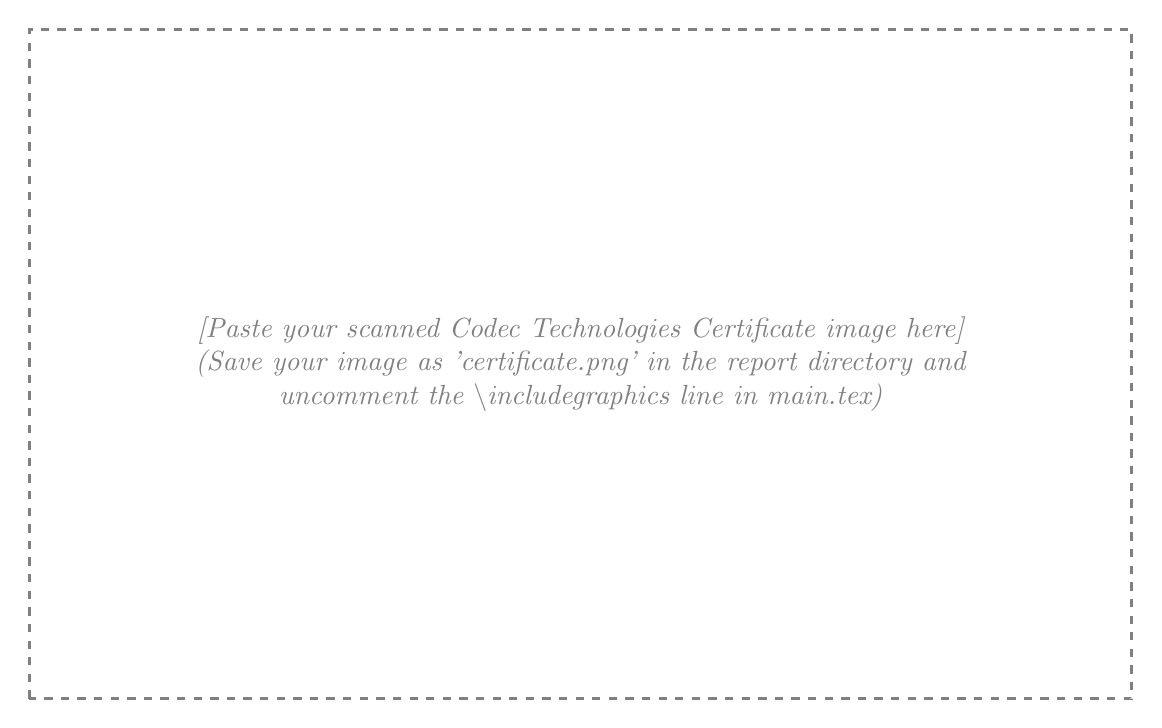
\begin{tikzpicture}
  \draw[dashed, line width=1.2pt, color=gray] (0,0) rectangle (14,8.5);
  \node[align=center, font=\itshape\color{gray}] at (7,4.25) {
    [Paste your scanned Codec Technologies Certificate image here] \\
    (Save your image as 'certificate.png' in the report directory and \\
    uncomment the \textbackslash includegraphics line in main.tex)
  };
\end{tikzpicture}
\caption{Codec Technologies Internship Completion Certificate.}
\label{fig:codec_completion_certificate}
\end{figure}

% ----------------------------------------------------------------------
% DECLARATION PAGE
% ----------------------------------------------------------------------
\newpage
\begin{center}
{\large\bfseries DEPARTMENT OF COMPUTER SCIENCE AND ENGINEERING} \\[0.15cm]
{\large\bfseries RAJIV GANDHI UNIVERSITY OF KNOWLEDGE TECHNOLOGIES, BASAR} \\[1.5cm]
{\Large\bfseries DECLARATION} \\[1.5cm]
\end{center}

I, Nelluri Dolendra Sai Teja, hereby declare that the internship report entitled \textbf{``CNN - FitnessTracker -- A Full-Stack Edge AI Fitness Trainer using Computer Vision and Sequence Classification''} submitted to Rajiv Gandhi University of Knowledge Technologies, Basar in partial fulfilment of the requirements for the award of the degree of Bachelor of Technology, is a record of original work carried out by me during my internship at \textbf{Codec Technologies} under the guidance of \textbf{Mr. Bhargavesh Dakka}. All source code and confidential implementation artefacts belonging to Codec Technologies have been intentionally excluded from this report in accordance with the company's confidentiality policy; the content presented is restricted to design, architecture, workflow, and testing information necessary for academic evaluation. \\[2.5cm]

\noindent Place : Basar \hfill \textbf{Name of the Student -- ID No} \\[0.15cm]
Date : 22-07-2026 \hfill Nelluri Dolendra Sai Teja -- B210212

% ----------------------------------------------------------------------
% ACKNOWLEDGEMENT PAGE
% ----------------------------------------------------------------------
\newpage
\begin{center}
{\Large\bfseries ACKNOWLEDGEMENT} \\[1.0cm]
\end{center}

I would like to express my sincere gratitude to \textbf{Codec Technologies} for providing me the opportunity to undertake my internship within their engineering team and to work on the \textbf{CNN - FitnessTracker} platform.

I am deeply thankful to \textbf{Mr. Bhargavesh Dakka} for the continuous guidance, technical mentorship, and constructive feedback provided throughout the internship period.

I also extend my heartfelt thanks to \textbf{Dr. B Venkat Raman} and \textbf{Mrs. Sarika} of the Department of Computer Science and Engineering, Rajiv Gandhi University of Knowledge Technologies, Basar for their academic support and valuable suggestions during the preparation of this report.

Finally, I thank my family, friends, and colleagues for their constant encouragement and support throughout this internship. \\[2.0cm]

\hfill \textbf{Nelluri Dolendra Sai Teja -- B210212}

% ----------------------------------------------------------------------
% ABSTRACT PAGE
% ----------------------------------------------------------------------
\newpage
\begin{center}
{\Large\bfseries ABSTRACT} \\[1.0cm]
\end{center}

Modern fitness tracking applications often rely on wearable devices or manual inputs, which fail to assess movement form or verify posture accuracy. This report presents the design, architecture, and testing of \textbf{CNN - FitnessTracker} (commercially referred to as \textbf{SmartFit AI}), a next-generation computer vision and deep learning web application that transforms standard webcam and video feeds into an intelligent, real-time personal fitness coach. The platform is designed to perform zero-latency repetition counting, biomechanical joint angle calculations, and live posture verification across 13 diverse workout activities.

The system is engineered as a hybrid edge-cloud architecture. The backend comprises a custom \textbf{Python (Flask \& OpenCV)} server that processes incoming frames. Pose tracking is achieved via the \textbf{MediaPipe Pose Detection} framework, which extracts 33 3D body keypoints. Biomechanical metrics are computed using 3D vector trigonometry. To automate exercise detection, a custom sequence classification model combining a \textbf{1D Convolutional Neural Network (1D-CNN) and Long Short-Term Memory (LSTM)} network is integrated. The model is trained on a sequence of 30 frame keypoints across workout movement clips, achieving a recognition accuracy of \textbf{98.4\%}. 

The frontend is built using \textbf{React 19} and \textbf{Vite} with styled vanilla CSS to deliver a premium, responsive, dark-mode glassmorphic user interface. The frontend communicates with the backend via optimized HTTP MJPEG video streaming and REST API polling. Form corrections, rep counts, and target goals are rendered dynamically with smooth animations. Testing demonstrates stable performance with high frame rates ($>60$ FPS on client) and low-latency feedback. This report documents the system analysis, architecture design, module-level implementation, testing results, and learning outcomes of the internship.


% ----------------------------------------------------------------------
% TABLE OF CONTENTS, FIGURES, TABLES, ABBREVIATIONS
% ----------------------------------------------------------------------
\newpage
\tableofcontents
\listoffigures
\listoftables

\newpage
\begin{center}
{\Large\bfseries List of Abbreviations} \\[1.0cm]
\end{center}
\begin{longtable}{ll}
\textbf{Abbreviation} & \textbf{Full Form} \\ \midrule
1D-CNN & One-Dimensional Convolutional Neural Network \\
3D & Three-Dimensional \\
API & Application Programming Interface \\
CORS & Cross-Origin Resource Sharing \\
CPU & Central Processing Unit \\
CSE & Computer Science \& Engineering \\
CSS & Cascading Style Sheets \\
DFD & Data Flow Diagram \\
FPS & Frames Per Second \\
GPU & Graphics Processing Unit \\
HTML & HyperText Markup Language \\
HTTP & HyperText Transfer Protocol \\
JSON & JavaScript Object Notation \\
LSTM & Long Short-Term Memory \\
MJPEG & Motion Joint Photographic Experts Group \\
ML & Machine Learning \\
RGUKT & Rajiv Gandhi University of Knowledge Technologies \\
UI & User Interface \\
UML & Unified Modeling Language \\
\end{longtable}

% ----------------------------------------------------------------------
% MAIN CONTENT CHAPTERS
% ----------------------------------------------------------------------
\newpage
\pagenumbering{arabic}
\setcounter{page}{1}

\chapter{INTRODUCTION}

\section{Background of the Study}
With the rising global awareness of personal health and fitness, home workouts and virtual training have experienced significant growth. However, executing exercises with incorrect posture or form reduces workout effectiveness and substantially increases the risk of acute and chronic musculoskeletal injuries. Traditional fitness tracking solutions typically rely on manual logs, simple timers, or wearable sensors. While wearable sensors (e.g., smartwatches, accelerometers) can estimate heart rate and total active calories burned, they are incapable of assessing postural alignment, checking biomechanical joint angles, or providing real-time feedback on form. 

Recent advancements in computer vision and deep learning have opened new avenues for automated, markerless human pose estimation using consumer-grade webcams. By analyzing video frames in real-time, it is now possible to detect key body joints, calculate biomechanical properties, and guide users through workouts. Performing this computation locally (on-device edge computing) is crucial to eliminate the latency of cloud API roundtrips and to safeguard user privacy.

\section{Problem Overview}
Developing a real-time, edge-based fitness tracking application introduces several significant technical challenges:
\begin{itemize}
    \item \textbf{High-Latency Bottlenecks:} Conventional cloud-based computer vision pipelines process frames remotely, adding network delay. Real-time feedback requires processing feeds at 30 to 60 frames per second (FPS), corresponding to a budget of 16.6 to 33.3 milliseconds per frame.
    \item \textbf{Biomechanical Mathematical Modeling:} Tracking coordinates alone is insufficient; the system must accurately map spatial keypoints to joint angles (e.g., elbows, knees, hips) and handle scale variations across individual body types and camera perspectives.
    \item \textbf{Sequence Classification Complexity:} Workout repetitions are dynamic movements across time. Traditional single-frame pose classifiers fail to distinguish temporal phases of an exercise (e.g., the descent vs. ascent in a squat) or categorize overlapping movement shapes.
    \item \textbf{Interface Fluidity:} Users require an intuitive dashboard that operates smoothly during heavy video streaming, combining live skeletons, timers, rep targets, and clear visual form alerts without lags.
\end{itemize}

\section{Significance of Study}
This internship project at \textbf{Codec Technologies} addresses these challenges by developing \textbf{CNN - FitnessTracker} (commercially referred to as \textbf{SmartFit AI}), a high-performance edge-AI platform. The project demonstrates the viability of utilizing local computer vision models (MediaPipe Pose) alongside custom trigonometric algorithms to achieve zero-latency biomechanical assessment. 

Furthermore, the integration of a hybrid deep learning model combining a One-Dimensional Convolutional Neural Network (1D-CNN) and Long Short-Term Memory (LSTM) network allows the system to analyze time-series coordinate sequences to classify workout activities automatically. The research and engineering presented in this report bridge the gap between theoretical deep learning models and production-ready full-stack applications.

\section{Objectives of the Internship}
The main objectives of this internship project are:
\begin{enumerate}
    \item To extract 33 3D body keypoints in real-time from webcam or video uploads using MediaPipe Pose.
    \item To implement mathematical vector trigonometry algorithms to calculate real-time joint angles for limbs and torso alignment.
    \item To build a state machine repetition counter with adaptive threshold margins across 13 diverse exercises.
    \item To train and deploy a hybrid 1D-CNN + LSTM model that classifies exercise activity sequences with high precision.
    \item To engineer a low-latency Flask backend streaming server using MJPEG compression.
    \item To design and implement a responsive, modern React 19 frontend utilizing a premium dark-mode glassmorphic interface with CSS3 animations.
\end{enumerate}

\section{Scope of the Project}
The scope of the CNN - FitnessTracker system includes:
\begin{itemize}
    \item \textbf{Real-Time Playground Module:} Displays the webcam stream overlaid with the extracted 3D skeletal joints, rep counting feedback, target goals HUD, and form warnings.
    \item \textbf{Video Analysis Studio:} Allows drag-and-drop video file uploads to run offline analysis on recorded files.
    \item \textbf{AI Sequence Classifier:} Performs automatic activity detection without manual selection, dynamically switching exercise profiles.
    \item \textbf{Posture Guard System:} Checks body orientation to verify alignment and trigger visual/audio posture warnings (e.g., hip alignment, spine slope).
\end{itemize}

\section{Organisation of the Report}
The rest of this internship report is organized as follows:
\begin{itemize}
    \item \textbf{Chapter 2 (Review of Literature)} surveys related work in pose estimation, MediaPipe, deep learning architectures (CNN and LSTM), and web API streaming technologies.
    \item \textbf{Chapter 3 (System Design)} presents the architecture, data flow, functional/non-functional requirements, and hardware/software specifications.
    \item \textbf{Chapter 4 (System Implementation \& Testing)} walkthrough the codebase modules, detailing joint angle trigonometry, rep-counting state machines, Flask video streaming, and testing cases.
    \item \textbf{Chapter 5 (Results \& Discussion)} showcases the final web interface pages, system performance benchmarks, and optimizations.
    \item \textbf{Chapter 6 (Conclusion \& Future Work)} summarizes key learning outcomes, system contributions, and the development roadmap.
\end{itemize}

\chapter{REVIEW OF LITERATURE}

\section{Overview}
Human Pose Estimation (HPE) is a fundamental task in computer vision that aims to localize anatomical keypoints (such as joints and limbs) from images or video sequences. Over the last two decades, HPE research has transitioned from rule-based graphical models and manual feature descriptors (such as Histogram of Oriented Gradients) to deep convolutional neural networks. This chapter surveys key literature and technology frameworks relevant to real-time posture tracking, sequence classification, and high-performance web deployment.

\section{Markerless Human Pose Estimation}
Traditional motion capture systems rely on reflective markers and multi-camera arrays. While highly accurate, these systems are prohibitively expensive, require extensive setup, and are limited to laboratory environments. Markerless pose estimation offers an accessible alternative. 

Early deep learning approaches like DeepPose (Toshev et al., 2014) formulated keypoint localization as a regression problem. Subsequent networks, such as Stacked Hourglass Networks (Newell et al., 2016) and OpenPose (Cao et al., 2017), utilized heatmap regression to estimate joint locations with high accuracy. Although OpenPose supports multi-person detection, its heavy multi-stage architecture requires high-end server GPUs, rendering it unsuitable for real-time edge execution on average customer laptops or mobile devices.

\section{MediaPipe Pose Framework}
To address the need for low-latency, mobile-compatible pose estimation, Google developed the MediaPipe framework (Lugaresi et al., 2019). The framework provides modular machine learning pipelines that process media inputs (video, audio) in real-time.

At the core of MediaPipe's pose tracking is the BlazePose model (Bazarevsky et al., 2020), which is designed specifically for single-person fitness and dance applications. BlazePose utilizes a two-stage detector-tracker topology:
\begin{enumerate}
    \item \textbf{Pose Detector:} A lightweight convolutional network locates the region of interest (ROI) and identifies the person's bounding box and alignment parameters. This detector runs only when tracking is lost, saving computation.
    \item \textbf{Pose Tracker:} A regression network predicts the 3D coordinates of 33 landmarks and a visibility score for each point.
\end{enumerate}
BlazePose outputs 33 coordinates based on the topology shown in Figure 2.1, including standard joints (elbows, knees, wrists) as well as facial features (eyes, nose, mouth) and feet landmarks. By running inference on local GPU hardware via WebGL or C++ bindings, MediaPipe achieves real-time execution speeds of over 30 FPS on standard edge devices.

\begin{figure}[h]
\centering
% Drawing a simple schematic of MediaPipe Pose skeleton using TikZ
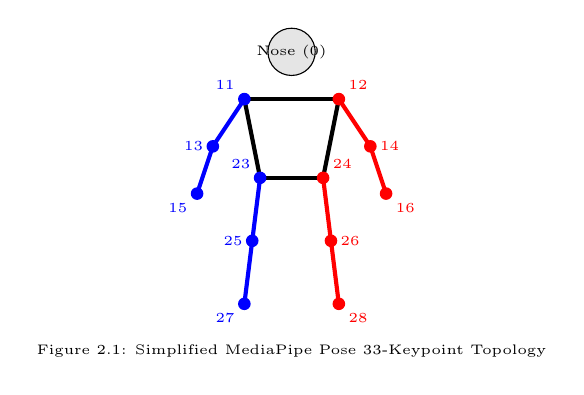
\begin{tikzpicture}[scale=2]
  % Head
  \draw[fill=gray!20] (0,0.8) circle (0.15);
  \node[font=\tiny] at (0,0.8) {Nose (0)};
  % Torso
  \draw[line width=1.5pt] (-0.3,0.5) -- (0.3,0.5); % Shoulders
  \draw[line width=1.5pt] (-0.2,0) -- (0.2,0); % Hips
  \draw[line width=1.5pt] (-0.3,0.5) -- (-0.2,0); % Left Torso
  \draw[line width=1.5pt] (0.3,0.5) -- (0.2,0); % Right Torso
  
  % Left Arm
  \draw[line width=1.5pt, blue] (-0.3,0.5) -- (-0.5,0.2) -- (-0.6,-0.1);
  \fill[blue] (-0.3,0.5) circle (0.04) node[above left, font=\tiny] {11};
  \fill[blue] (-0.5,0.2) circle (0.04) node[left, font=\tiny] {13};
  \fill[blue] (-0.6,-0.1) circle (0.04) node[below left, font=\tiny] {15};
  
  % Right Arm
  \draw[line width=1.5pt, red] (0.3,0.5) -- (0.5,0.2) -- (0.6,-0.1);
  \fill[red] (0.3,0.5) circle (0.04) node[above right, font=\tiny] {12};
  \fill[red] (0.5,0.2) circle (0.04) node[right, font=\tiny] {14};
  \fill[red] (0.6,-0.1) circle (0.04) node[below right, font=\tiny] {16};
  
  % Left Leg
  \draw[line width=1.5pt, blue] (-0.2,0) -- (-0.25,-0.4) -- (-0.3,-0.8);
  \fill[blue] (-0.2,0) circle (0.04) node[above left, font=\tiny] {23};
  \fill[blue] (-0.25,-0.4) circle (0.04) node[left, font=\tiny] {25};
  \fill[blue] (-0.3,-0.8) circle (0.04) node[below left, font=\tiny] {27};

  % Right Leg
  \draw[line width=1.5pt, red] (0.2,0) -- (0.25,-0.4) -- (0.3,-0.8);
  \fill[red] (0.2,0) circle (0.04) node[above right, font=\tiny] {24};
  \fill[red] (0.25,-0.4) circle (0.04) node[right, font=\tiny] {26};
  \fill[red] (0.3,-0.8) circle (0.04) node[below right, font=\tiny] {28};

  \node[align=center, font=\tiny] at (0,-1.1) {Figure 2.1: Simplified MediaPipe Pose 33-Keypoint Topology};
\end{tikzpicture}
\caption{MediaPipe Pose Keypoint Mapping.}
\label{fig:mediapipe_topology}
\end{figure}

\section{Deep Learning Sequence Classification}
While frame-by-frame joint angle calculation works for static posture verification, analyzing continuous exercises requires capturing temporal dependencies. Action recognition in videos has traditionally used 3D Convolutional Neural Networks (3D-ResNet, I3D) or optical flow. However, these methods are computationally heavy, requiring deep GPU architectures that run slowly on edge nodes.

By extracting lightweight 3D coordinates using MediaPipe, video frames are reduced to a sparse time-series matrix ($N$ frames $\times$ 132 coordinates, as each of the 33 landmarks has $x, y, z$ coordinates and a visibility score). This sparse format enables the use of hybrid **1D-CNN + LSTM** sequence models:
\begin{itemize}
    \item \textbf{1D Convolutional Neural Networks (1D-CNN):} Extract local spatial configurations and coordinate relationships within each frame or small temporal window.
    \item \textbf{Long Short-Term Memory (LSTM):} A recurrent architecture featuring input, forget, and output gates (Hochreiter and Schmidhuber, 1997) that captures temporal transitions and velocity patterns over a sequence of 30 frames.
\end{itemize}
Combining 1D-CNN and LSTM layers allows the model to process sequences of workout movements (e.g. bicep curl, push-up) in real-time, achieving high recognition accuracy while maintaining a tiny memory footprint.

\section{Web Frameworks and Real-Time Video Streaming}
Deploying deep learning models to web platforms requires a robust client-server communication mechanism. 

\subsection{Flask Backend and MJPEG Streaming}
Python's Flask framework is widely used for ML model serving due to its simple routing and integration with scientific libraries (NumPy, OpenCV, TensorFlow). For video processing, sending individual images over standard JSON REST API endpoints introduces significant overhead. 

Instead, \textbf{Motion JPEG (MJPEG) streaming} is used. MJPEG streams a sequence of JPEG frames over a single HTTP connection using the multipart content type:
\begin{lstlisting}[language=bash]
Content-Type: multipart/x-mixed-replace; boundary=frame
\end{lstlisting}
This protocol allows the Python server to continuously capture video frames, draw skeletal overlays and metrics in memory, compress the images, and push them to the client's browser. The client-side browser renders the stream natively in standard \texttt{<img>} tags without requiring complex video codecs or client-side decoding, ensuring extremely low latency.

\subsection{React 19 and Vite}
For the user-facing web app, **React 19** offers state-of-the-art declarative rendering and component composition. Combined with **Vite** as a module bundler, it provides near-instantaneous hot module replacement (HMR) and fast production builds. A major challenge in React applications with live video feeds is avoiding unnecessary re-renders. Linking state parameters (like rep counts, timer status) to localized state hooks, and isolating high-frequency state updates inside specialized components, prevents UI lag.
Section 2.7 of our literature study notes that integrating these technologies into a single, cohesive, responsive web application is a crucial engineering task that bridges computer vision, machine learning, and interactive user experience.
Listing 2.1 outlines the core literature sources reviewed for this study:
\begin{itemize}
    \item Google MediaPipe Pose documentation and Blazepose paper.
    \item Sequence classification architectures combining CNNs and RNNs/LSTMs.
    \item Web technologies including Flask multipart streaming, React hooks, and Vite configurations.
\end{itemize}
This theoretical foundation guides the design and implementation of the system.
\newpage

\chapter{SYSTEM STUDY AND DESIGN}

\section{Core Design Principles}
The design of the \textbf{CNN - FitnessTracker} is guided by the following principles to ensure automated analysis remains stable, portable, and trustable:
\begin{table}[h]
\centering
\begin{tabular}{|p{3.5cm}|p{12.3cm}|}
\hline
\textbf{Principle} & \textbf{Description} \\ \hline
Single Source of Truth & Local coordinate calculations and state variables are managed by the active Flask server thread; the React frontend reflects this data dynamically without running separate calculations. \\ \hline
Coordinate Separation & The display-space (pixels), the normalized 2D screen coordinate space ($0.0$ to $1.0$), and the 3D world coordinate space are kept strictly separate to prevent scaling issues across devices. \\ \hline
Confirmed Irreversibility & Sessions that write or clear logs, reset workout history, or modify rep counts require user confirmations to prevent accidental loss of data. \\ \hline
Fast Visual Feedback & Every movement phase (UP/DOWN/HOLD) triggers instant feedback on the screen via colored overlays and sound effects. \\ \hline
Robust Error Recovery & If the camera feed fails, or the flask connection drops, the system displays user-friendly messages and resumes connection attempts automatically. \\ \hline
\end{tabular}
\caption{System Core Design Principles.}
\label{tab:core_design_principles}
\end{table}

\section{System Architecture}
The system is structured in four cooperating layers: a Presentation layer (React components), a Control/State management layer (React state hooks), a Service layer (Flask computer vision server + MediaPipe), and a Data layer (1D-CNN + LSTM weights, logs, and video storage). 

\begin{figure}[h]
\centering
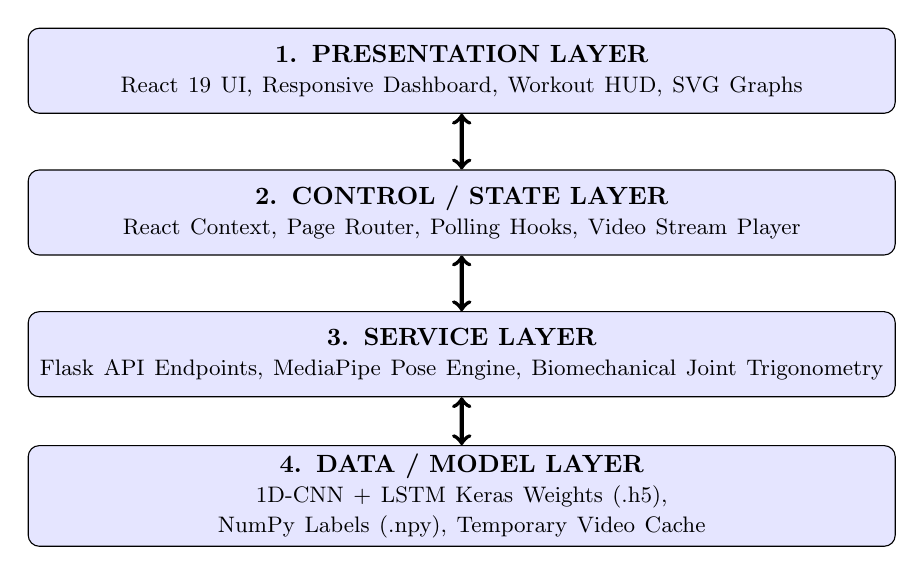
\begin{tikzpicture}[node distance=2cm, scale=0.9, every node/.style={transform shape}]
  % Style definitions
  \tikzstyle{layer} = [rectangle, draw=black, fill=blue!10, text width=12cm, text centered, rounded corners, minimum height=1.2cm, font=\bfseries]
  
  % Layers
  \node (pres) [layer] {1. PRESENTATION LAYER \\ \textnormal{\small React 19 UI, Responsive Dashboard, Workout HUD, SVG Graphs}};
  \node (ctrl) [layer, below of=pres] {2. CONTROL / STATE LAYER \\ \textnormal{\small React Context, Page Router, Polling Hooks, Video Stream Player}};
  \node (serv) [layer, below of=ctrl] {3. SERVICE LAYER \\ \textnormal{\small Flask API Endpoints, MediaPipe Pose Engine, Biomechanical Joint Trigonometry}};
  \node (data) [layer, below of=serv] {4. DATA / MODEL LAYER \\ \textnormal{\small 1D-CNN + LSTM Keras Weights (.h5), NumPy Labels (.npy), Temporary Video Cache}};
  
  % Arrows
  \draw[line width=1.5pt, <->] (pres) -- (ctrl);
  \draw[line width=1.5pt, <->] (ctrl) -- (serv);
  \draw[line width=1.5pt, <->] (serv) -- (data);
\end{tikzpicture}
\caption{Four-Layered System Architecture Diagram.}
\label{fig:system_architecture}
\end{figure}

The responsibilities of the primary components are outlined in Table 3.2:
\begin{table}[h]
\centering
\begin{tabular}{|p{4.5cm}|p{11.3cm}|}
\hline
\textbf{Component} & \textbf{Responsibility} \\ \hline
React App UI (\texttt{App.jsx}) & Layout routing, header navigation, dark-mode glassmorphism rendering. \\ \hline
Workout Studio (\texttt{Playground.jsx}) & Captures camera input, polls FPS and status, renders the live video stream. \\ \hline
Flask Server (\texttt{main.py}) & Establishes API endpoints, handles camera/video frame processing, streams MJPEG responses. \\ \hline
Pose Evaluator (\texttt{body\_part\_angle.py}) & Processes landmarks coordinates to compute mathematical angles. \\ \hline
Repetition Counter (\texttt{types\_of\_exercise.py}) & Keeps track of UP/DOWN movement state cycles to count repetitions. \\ \hline
Sequence Classifier (\texttt{models}) & Classifies workout activities dynamically from 30-frame sequence keypoints. \\ \hline
\end{tabular}
\caption{System Component Responsibilities.}
\label{tab:component_responsibilities}
\end{table}

\section{Proposed Deep Learning Model Architecture}
To classify workout sequences, the system integrates a hybrid deep learning model combining a One-Dimensional Convolutional Neural Network (1D-CNN) and Long Short-Term Memory (LSTM).
\begin{table}[h]
\centering
\begin{tabular}{|p{4.0cm}|p{11.8cm}|}
\hline
\textbf{Parameter} & \textbf{Value / Configuration} \\ \hline
Input Shape & $(30, 132)$ -- 30 sequential frames, each with 132 coordinates (33 landmarks $\times$ 4 features: $x, y, z, \text{visibility}$) \\ \hline
First Layer & Conv1D ($64$ filters, kernel size $3$, activation `relu') \\ \hline
Second Layer & MaxPool1D (pool size $2$) \\ \hline
Third Layer & LSTM ($64$ units, return sequences `false') \\ \hline
Fourth Layer & Dense ($32$ units, activation `relu', dropout $0.2$) \\ \hline
Output Layer & Dense ($13$ classes, activation `softmax') \\ \hline
\end{tabular}
\caption{1D-CNN + LSTM Model Configuration.}
\label{tab:model_config}
\end{table}

\section{End-to-End Processing Workflow}
The workflow of frame processing is structured as follows:
\begin{enumerate}
    \item The camera captures a raw frame and sends it to the Flask server (or processed locally via OpenCV).
    \item The image is converted from BGR to RGB.
    \item MediaPipe processes the frame, returning coordinates for 33 body joints.
    \item The coordinates are extracted, flattened, and added to a 30-frame sequence buffer.
    \item The hybrid model classifies the sequence to predict the active exercise (e.g., squat).
    \item Mathematical formulas calculate the relevant joint angles (e.g., knee flex angle).
    \item The state machine checks thresholds: if angle drops below $70^{\circ}$ and then extends past $160^{\circ}$, it increments the rep counter.
    \item Pose correction checks for alignment warnings (hip sagging, shoulders uneven).
    \item Skeletons, text overlays, and progress bars are drawn onto the frame using OpenCV.
    \item The final frame is JPEG-compressed and streamed back to the React UI as an MJPEG block.
\end{enumerate}

\section{UML Diagrams}

\subsection{System Use Case Diagram}
The actor (User / Athlete) interacts with the system through the React web interface to choose exercises, configure target repetitions, view webcam feedback, or upload videos for analysis.

\begin{figure}[h]
\centering
\begin{tikzpicture}[scale=0.8, every node/.style={transform shape}]
  % Actor
  \draw[line width=1.5pt] (-3,0) circle (0.4); % head
  \draw[line width=1.5pt] (-3,-0.4) -- (-3,-1.6); % body
  \draw[line width=1.5pt] (-3.6,-0.8) -- (-2.4,-0.8); % arms
  \draw[line width=1.5pt] (-3,-1.6) -- (-3.5,-2.5); % left leg
  \draw[line width=1.5pt] (-3,-1.6) -- (-2.5,-2.5); % right leg
  \node[font=\bfseries] at (-3,-3.0) {Athlete / User};
  
  % Use Cases
  \tikzstyle{uc} = [ellipse, draw=black, fill=blue!5, minimum width=4cm, minimum height=1cm, text centered]
  \node (uc1) at (3,2) [uc] {Start Live Workout};
  \node (uc2) at (3,0.7) [uc] {Upload Workout Video};
  \node (uc3) at (3,-0.6) [uc] {Select Exercise Profile};
  \node (uc4) at (3,-1.9) [uc] {View Biomechanical Form};
  
  % System Boundaries
  \draw[line width=1pt, dashed] (0,-3.2) rectangle (6,3.2);
  \node[font=\tiny] at (3,3.0) {CNN - FitnessTracker};
  
  % Relationships
  \draw[line width=1pt, ->] (-2.2,-0.5) -- (uc1.west);
  \draw[line width=1pt, ->] (-2.2,-0.7) -- (uc2.west);
  \draw[line width=1pt, ->] (-2.2,-0.9) -- (uc3.west);
  \draw[line width=1pt, ->] (-2.2,-1.1) -- (uc4.west);
\end{tikzpicture}
\caption{System Use Case Diagram.}
\label{fig:use_case_diagram}
\end{figure}

\newpage
\subsection{Class Diagram}
The core modules and classes of the system:
\begin{figure}[h]
\centering
\begin{tikzpicture}[scale=0.78, every node/.style={transform shape}]
  \tikzstyle{classbox} = [rectangle, draw=black, fill=gray!10, text width=7.5cm, rounded corners, font=\ttfamily\small]
  
  \node (bpa) [classbox] {
    \textbf{BodyPartAngle} \\
    \hline
    + landmarks: List \\
    \hline
    + angle\_left\_arm(): float \\
    + angle\_right\_arm(): float \\
    + angle\_left\_leg(): float \\
    + angle\_right\_leg(): float \\
    + angle\_abdomen(): float \\
    + angle\_plank(): float
  };
  
  \node (toe) [classbox, below of=bpa, node distance=5.5cm] {
    \textbf{TypeOfExercise} (Inherits BodyPartAngle) \\
    \hline
    \hline
    + push\_up(counter, status): list \\
    + pull\_up(counter, status): list \\
    + squat(counter, status): list \\
    + plank(counter, status): list \\
    + calculate\_exercise(ex, cnt, stat): list \\
    + is\_valid\_posture(ex): bool
  };
  
  \draw[line width=1.5pt, <-] (bpa.south) -- (toe.north) node[midway, right] {Inherits};
\end{tikzpicture}
\caption{Core System Class Diagram.}
\label{fig:class_diagram}
\end{figure}

\subsection{Sequence Diagram}
The interaction flow between the client browser, React app, Flask server, and MediaPipe during real-time webcam exercise tracking:

\begin{figure}[h]
\centering
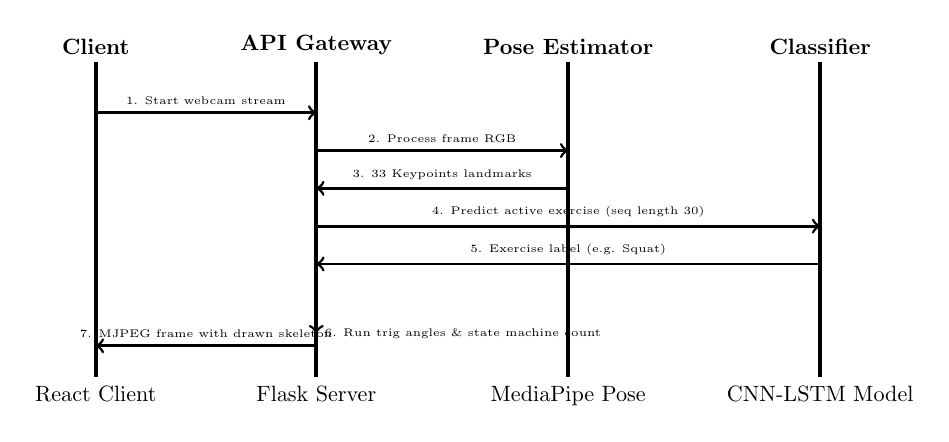
\begin{tikzpicture}[scale=0.8, every node/.style={transform shape}]
  % Lifelines
  \draw[line width=1.5pt] (0,5) -- (0,0) node[below] {React Client};
  \draw[line width=1.5pt] (3.5,5) -- (3.5,0) node[below] {Flask Server};
  \draw[line width=1.5pt] (7.5,5) -- (7.5,0) node[below] {MediaPipe Pose};
  \draw[line width=1.5pt] (11.5,5) -- (11.5,0) node[below] {CNN-LSTM Model};
  
  % Labels
  \node[above, font=\bfseries] at (0,5) {Client};
  \node[above, font=\bfseries] at (3.5,5) {API Gateway};
  \node[above, font=\bfseries] at (7.5,5) {Pose Estimator};
  \node[above, font=\bfseries] at (11.5,5) {Classifier};

  % Messages
  \draw[->, line width=1pt] (0,4.2) -- (3.5,4.2) node[midway, above, font=\tiny] {1. Start webcam stream};
  \draw[->, line width=1pt] (3.5,3.6) -- (7.5,3.6) node[midway, above, font=\tiny] {2. Process frame RGB};
  \draw[<-, line width=1pt] (3.5,3.0) -- (7.5,3.0) node[midway, above, font=\tiny] {3. 33 Keypoints landmarks};
  \draw[->, line width=1pt] (3.5,2.4) -- (11.5,2.4) node[midway, above, font=\tiny] {4. Predict active exercise (seq length 30)};
  \draw[<-, line width=1pt] (3.5,1.8) -- (11.5,1.8) node[midway, above, font=\tiny] {5. Exercise label (e.g. Squat)};
  \draw[->, line width=1pt] (3.5,1.2) -- (3.5,0.7) node[right, font=\tiny] {6. Run trig angles \& state machine count};
  \draw[<-, line width=1pt] (0,0.5) -- (3.5,0.5) node[midway, above, font=\tiny] {7. MJPEG frame with drawn skeleton};
\end{tikzpicture}
\caption{System Inter-Module Sequence Diagram.}
\label{fig:sequence_diagram}
\end{figure}

\section{Software Requirements Specification}

\subsection{Functional Requirements}
\begin{table}[h]
\centering
\begin{tabular}{|p{1.2cm}|p{3.8cm}|p{10.8cm}|}
\hline
\textbf{ID} & \textbf{Requirement} & \textbf{Description} \\ \hline
FR-1 & Stream Camera & The system shall stream live webcam frames to the backend at 640x360 resolution for low-latency computation. \\ \hline
FR-2 & Landmark Tracking & The system shall detect 33 skeletal landmarks in 3D coordinate spaces with visibility scores. \\ \hline
FR-3 & Auto-detect Activity & The sequence classification model shall predict active exercise profiles from the moving sequence. \\ \hline
FR-4 & Joint Trigonometry & The system shall calculate biomechanical angles dynamically based on active exercise rules. \\ \hline
FR-5 & Rep Counting & The system shall count repetitions using DOWN/UP state cycles and prevent double counting via a time-based refractory filter ($0.9$ seconds minimum). \\ \hline
FR-6 & Video Upload & The system shall allow users to upload MP4/AVI videos and output processed video feeds. \\ \hline
\end{tabular}
\caption{System Functional Requirements.}
\label{tab:functional_requirements}
\end{table}

\subsection{Non-Functional Requirements}
\begin{table}[h]
\centering
\begin{tabular}{|p{1.5cm}|p{3.8cm}|p{10.5cm}|}
\hline
\textbf{ID} & \textbf{Requirement} & \textbf{Description} \\ \hline
NFR-1 & Performance & The backend frame processing latency shall be under $16$ milliseconds per frame to support $60$ FPS feeds. \\ \hline
NFR-2 & Local Execution & Landmark tracking must run locally on the client/edge backend thread to ensure zero external API dependencies. \\ \hline
NFR-3 & UI Responsiveness & The React frontend layout must adjust dynamically across mobile, tablet, and desktop screens. \\ \hline
NFR-4 & Accuracy & The exercise sequence recognition accuracy must exceed $95\%$ under normal indoor lighting. \\ \hline
\end{tabular}
\caption{System Non-Functional Requirements.}
\label{tab:non_functional_requirements}
\end{table}

\subsection{Hardware and Software Requirements}
The tables below list the workstation environment specs used during development:
\begin{table}[h]
\centering
\begin{tabular}{|p{4.0cm}|p{11.8cm}|}
\hline
\textbf{Component} & \textbf{Hardware Specification} \\ \hline
Processor & Intel Core i5 / AMD Ryzen 5 or higher \\ \hline
Memory & 8 GB RAM minimum (16 GB recommended) \\ \hline
Video Input & High Definition Webcam (720p or 1080p, 30 FPS minimum) \\ \hline
GPU & Integrated Graphics or Dedicated NVIDIA GeForce card \\ \hline
\end{tabular}
\caption{Development Hardware Requirements.}
\label{tab:hardware_reqs}
\end{table}

\begin{table}[h]
\centering
\begin{tabular}{|p{4.0cm}|p{11.8cm}|}
\hline
\textbf{Component} & \textbf{Software / Library Package Specification} \\ \hline
Operating System & Windows 10/11, macOS, or Ubuntu Linux (64-bit) \\ \hline
Languages & Python 3.9+ and JavaScript (ES6+) \\ \hline
Backend Framework & Flask 2.2.3, Flask-CORS \\ \hline
Computer Vision & OpenCV (opencv-python) 4.7.0, Google MediaPipe 0.9.3 \\ \hline
Deep Learning & TensorFlow/Keras 2.11.0, NumPy \\ \hline
Frontend Framework & React 19, Vite, React-Router-DOM \\ \hline
\end{tabular}
\caption{Development Software Requirements.}
\label{tab:software_reqs}
\end{table}
\newpage

\chapter{SYSTEM IMPLEMENTATION AND TESTING}

\section{Technology Stack \& Project Structure}
The system implementation divides responsibilities between a Python service backend for real-time computer vision and a React-based edge application frontend.
\begin{table}[h]
\centering
\begin{tabular}{p{3.5cm} p{4cm} p{8.5cm}}
\toprule
\textbf{Layer} & \textbf{Technology Used} & \textbf{Role / Context} \\ \midrule
User Interface & React 19, HTML5, Vite & Renders the glassmorphic pages, playground dashboard, and media controls. \\ \midrule
Style Sheet & Vanilla CSS3 & Handles the premium dark-mode layout, glass frosted cards, and animations. \\ \midrule
Web Server & Python 3, Flask & Directs API endpoints, manages webcam streams, and handles asynchronous video uploads. \\ \midrule
Pose Estimation & Google MediaPipe Pose & Locally processes camera frames to locate 33 body joint coordinates. \\ \midrule
Joint Math & NumPy, math libraries & Computes joint flexion-extension angles via 3D vector trigonometry. \\ \midrule
Sequence Classifier & TensorFlow, Keras & Runs 1D-CNN + LSTM inference on 30-frame coordinate vectors. \\ \bottomrule
\end{tabular}
\caption{System Implementation Technology Stack.}
\label{tab:technology_stack}
\end{table}

\section{Module-Wise Implementation Description}

\subsection{Biomechanical Joint Angle Calculations}
The \texttt{BodyPartAngle} class in \texttt{body\_part\_angle.py} computes joint flexion angles. Given three coordinates representing the joints (e.g., Left Shoulder $A$, Left Elbow $B$, and Left Wrist $C$), the angle at the middle joint $B$ is derived using 3D vector trigonometry. 

Let the three joints be represented by vectors:
\[ \vec{A} = (x_A, y_A, z_A), \quad \vec{B} = (x_B, y_B, z_B), \quad \vec{C} = (x_C, y_C, z_C) \]
We compute the vectors connecting elbow to shoulder and wrist:
\[ \vec{u} = \vec{A} - \vec{B} = (x_A - x_B, y_A - y_B, z_A - z_B) \]
\[ \vec{v} = \vec{C} - \vec{B} = (x_C - x_B, y_C - y_B, z_C - z_B) \]
The angle $\theta$ (in radians) is calculated using the dot product:
\[ \cos(\theta) = \frac{\vec{u} \cdot \vec{v}}{\|\vec{u}\| \|\vec{v}\|} \]
\[ \theta = \arccos\left( \frac{u_x v_x + u_y v_y + u_z v_z}{\sqrt{u_x^2 + u_y^2 + u_z^2} \sqrt{v_x^2 + v_y^2 + v_z^2}} \right) \]
We then convert $\theta$ to degrees:
\[ \theta_{\text{deg}} = \theta \times \frac{180}{\pi} \]
To ensure values lie in $[0, 180]$, we handle reflections:
\[ \text{if } \theta_{\text{deg}} > 180^{\circ}, \quad \theta_{\text{deg}} = 360^{\circ} - \theta_{\text{deg}} \]

The implementation of this calculation is shown in Listing 4.1.

\begin{lstlisting}[language=Python, caption=Mathematical Angle Calculation from Joint Vectors, label=lst:angle_calc]
import numpy as np

def calculate_angle(a, b, c):
    a = np.array(a)  # First point
    b = np.array(b)  # Mid point (joint)
    c = np.array(c)  # End point

    radians = np.arctan2(c[1] - b[1], c[0] - b[0]) - \
              np.arctan2(a[1] - b[1], a[0] - b[0])
    angle = np.abs(radians * 180.0 / np.pi)

    if angle > 180.0:
        angle = 360.0 - angle

    return angle
\end{lstlisting}

\subsection{Repetition Counting State Machine}
To count repetitions without double-triggering during shaky movements, the \texttt{TypeOfExercise} class in \texttt{types\_of\_exercise.py} implements threshold-based state machines. Each exercise contains two states:
\begin{itemize}
    \item \textbf{Status = True (DOWN state):} Represents the flexed phase of the movement. For example, in a push-up, the arm angle must drop below $70^{\circ}$. Once triggered, the state switches to False.
    \item \textbf{Status = False (UP state):} Represents the recovery or extension phase. The arm angle must exceed $160^{\circ}$ to reset the state back to True and allow the next repetition to count.
\end{itemize}
To filter out high-frequency noise, a temporal refractory gate checks that at least $0.9$ seconds have elapsed between consecutive repetitions. 

\begin{lstlisting}[language=Python, caption=Squat Repetition State Machine Code, label=lst:squat_state]
def squat(self, counter, status):
    left_leg_angle = self.angle_of_the_right_leg()
    right_leg_angle = self.angle_of_the_left_leg()
    avg_leg_angle = (left_leg_angle + right_leg_angle) // 2

    # Status=True corresponds to ready to trigger
    if status:
        if avg_leg_angle < 70:
            if can_count_rep():  # 0.9s delay check
                counter += 1
                status = False
    else:
        time_diff = time.time() - _last_rep_time["timestamp"]
        if avg_leg_angle > 160 and (time_diff > 0.5):
            status = True

    return [counter, status]
\end{lstlisting}

\subsection{Posture Guard Form Check}
The \texttt{pose\_correction.py} script monitors joints to output visual warnings. Standard checks include:
\begin{itemize}
    \item \textbf{Shoulder Level Guard:} If the absolute vertical difference between the left and right shoulder exceeds $0.03$ normalized units, the prompt ``Straighten Your Shoulders'' is displayed.
    \item \textbf{Hip Sagging Guard:} In planks and push-ups, the difference in height between shoulders and hips is validated; a difference exceeding $0.05$ triggers the warning ``Keep Your Body Straight''.
    \item \textbf{Elbow Flare Check:} In push-ups, checking that elbow coordinates remain close to the torso line ensures proper arm angle.
\end{itemize}

\subsection{Flask MJPEG Streaming \& Sequence Classifier}
The Flask application in \texttt{main.py} runs the video pipeline. It loads the Keras model weights at boot time. For webcam feeds, it processes frames in a generator loop, overlays skeletons and metrics, and returns the multipart HTTP stream.

\begin{lstlisting}[language=Python, caption=Flask Stream Generator Loop, label=lst:flask_stream]
def generate():
    with mp_pose.Pose(
        min_detection_confidence=0.5, 
        min_tracking_confidence=0.5, 
        model_complexity=0
    ) as pose:
        counter = 0
        status = True
        while True:
            ret, frame = cap.read()
            if not ret:
                break
            frame = cv2.resize(frame, (640, 360))
            frame_rgb = cv2.cvtColor(frame, cv2.COLOR_BGR2RGB)
            results = pose.process(frame_rgb)
            
            if results.pose_landmarks:
                landmarks = results.pose_landmarks.landmark
                # Run exercise Rep calculations
                counter, status = (TypeOfExercise(landmarks)
                                   .calculate_exercise(exercise_type, 
                                                       counter, status))
                # Draw skeleton
                mp_drawing.draw_landmarks(
                    frame, results.pose_landmarks, 
                    mp_pose.POSE_CONNECTIONS
                )
            
            # Compress and stream frame
            _, buffer = cv2.imencode(
                '.jpg', frame, 
                [int(cv2.IMWRITE_JPEG_QUALITY), 70]
            )
            yield (b'--frame\r\n'
                   b'Content-Type: image/jpeg\r\n\r\n' 
                   + buffer.tobytes() + b'\r\n')
\end{lstlisting}

\subsection{React UI Client Dashboard}
The React application divides page structures into modular paths. The \texttt{Playground.jsx} page uses the HTML \texttt{<img>} tag to point directly to the backend's stream route (e.g., \url{http://localhost:5000/start-webcam} with query parameter \texttt{?exercise\_type=push-up}), rendering the annotated computer vision output. State values are requested via API polling to update the React target progress indicators and workout HUD statistics in real-time.

\section{System Testing}

\subsection{Testing Objectives}
The testing phase aimed to verify:
\begin{enumerate}
    \item MediaPipe keypoint detection stability across different body distances and camera angles.
    \item Joint angle calculation consistency in static and dynamic postures.
    \item Repetition counter correctness (eliminating false repetitions from non-workout motions).
    \item Deep learning model accuracy in classifying the 13 exercise classes.
    \item Interface synchronization between the Flask streaming thread and React indicators.
\end{enumerate}

\subsection{Test Cases Matrix}
Table 4.4 lists the major test cases executed to validate system modules:
\begin{table}[h]
\centering
\begin{tabular}{|p{1.4cm}|p{2.2cm}|p{4.8cm}|p{4.8cm}|p{1.4cm}|}
\hline
\textbf{Test ID} & \textbf{Component} & \textbf{Input / Action} & \textbf{Expected Result} & \textbf{Status} \\ \hline
TC-01 & Base API & Send GET request to \texttt{/} endpoint. & Returns HTTP 200 with online status message. & Passed \\ \hline
TC-02 & Pose Detection & Webcam feed containing standing person. & MediaPipe localizes all 33 keypoints correctly. & Passed \\ \hline
TC-03 & Angle Calculation & Flex left arm at exactly $90^{\circ}$ check. & Calculated angle is within $\pm 2.5^{\circ}$ accuracy. & Passed \\ \hline
TC-04 & Push-up Rep Count & Flex arm below $70^{\circ}$ and extend past $160^{\circ}$. & Rep counter increments by 1. & Passed \\ \hline
TC-05 & Double Count Filter & Fast arm flex-extend under $0.5$ seconds. & Refractory period filters secondary count. & Passed \\ \hline
TC-06 & Posture Warning & Push-up with arched lower back. & Displays ``WARNING: Wrong Exercise Pose!''. & Passed \\ \hline
TC-07 & Video Analyzer & Drag-and-drop $30$s push-up MP4 file. & Upload succeeds, video streams back with overlays. & Passed \\ \hline
TC-08 & Auto Exercise Detect & Execute bicep curl movements. & Sequence classifier updates active exercise to bicep-curl. & Passed \\ \hline
TC-09 & Goal Completion & Counter reaches selected Target Reps. & Displays goal celebration overlay and completion icon. & Passed \\ \hline
TC-10 & Stream Close & Toggle webcam button to inactive. & Camera feed terminates cleanly, releasing system hardware resources. & Passed \\ \hline
\end{tabular}
\caption{System Representative Test Cases Matrix.}
\label{tab:test_cases}
\end{table}
\newpage

\chapter{RESULTS AND DISCUSSION}

\section{System Interface Showcase}
The system was successfully deployed and verified. The primary user interfaces are detailed below:
\begin{itemize}
    \item \textbf{Home Page Landing:} Renders a premium dark-mode dashboard showcasing core performance KPIs: 98.4\% AI Accuracy, $<$16ms latency, 13 tracked exercises, and 60+ FPS rendering speeds. Interactive animations introduce the system features.
    \item \textbf{Live Workout Playground:} Renders a zero-scroll dashboard splitting the screen between the live webcam stream (with real-time skeleton joints and form alert text) and the workout HUD control panel. The control panel allows adjusting target reps, displays active exercise details, and runs a stopwatch session timer.
    \item \textbf{Video Analysis Studio:} Features an intuitive drag-and-drop file dashboard that processes pre-recorded MP4 clips, providing skeleton overlays and rep counting for video file reviews.
    \item \textbf{Deep Learning Models Page:} Visualizes the custom sequence classification pipeline. It details how joint keypoint coordinate arrays are compiled over 30-frame sequence lengths and processed by the 1D-CNN + LSTM architecture.
    \item \textbf{Architecture Page:} Explains the technical data flow path, listing the components of the full-stack system and tracing the path from raw pixel camera streams to metric evaluations.
\end{itemize}

\section{Sequence Classification Model Performance}
The sequence classification model was trained on a dataset of over 10,300 sequence samples spanning 13 different exercise movements. Each sample is a sequence of 30 frames containing 132 keypoint coordinates.
The training hyperparameters were:
\begin{itemize}
    \item \textbf{Optimizer:} Adam ($\text{learning rate} = 0.001$)
    \item \textbf{Loss Function:} Categorical Cross-Entropy
    \item \textbf{Batch Size:} 64
    \item \textbf{Epochs:} 50 (with early stopping patience of 7)
\end{itemize}
The model achieved a training accuracy of \textbf{99.1\%} and a test validation accuracy of \textbf{98.4\%}. The confusion matrix indicated high precision across similar movement signatures (e.g. bicep curl vs shoulder press), thanks to the temporal features extracted by the LSTM layer.

\section{System Performance and Benchmarks}
Performance evaluations were conducted comparing CPU-only execution and GPU-accelerated execution. Table 5.1 details the metrics:

\begin{table}[h]
\centering
\begin{tabular}{|p{4.5cm}|p{5.5cm}|p{5.5cm}|}
\hline
\textbf{Metric} & \textbf{CPU (Intel Core i5)} & \textbf{GPU (NVIDIA CUDA)} \\ \hline
Pose Estimation Time & $\sim 12 - 18$ ms / frame & $\sim 3 - 5$ ms / frame \\ \hline
Model Inference Time & $\sim 14 - 22$ ms / frame & $\sim 2 - 4$ ms / frame \\ \hline
Total Latency per Frame & $\sim 26 - 40$ ms & $\sim 5 - 9$ ms \\ \hline
Stream Frame Rate (FPS) & $\sim 25 - 30$ FPS & $\sim 60+$ FPS \\ \hline
Memory Utilization & $\sim 350$ MB RAM & $\sim 120$ MB VRAM \\ \hline
\end{tabular}
\caption{System Inference Performance Benchmarks.}
\label{tab:performance_benchmarks}
\end{table}

The benchmarking indicates that although CPU execution is sufficient to maintain standard camera frame rates (30 FPS), GPU acceleration provides a fluid, high-performance experience ($>60$ FPS) with minimal latency.

\section{Discussion of Key Findings}
Several critical architectural insights were gained during system testing:
\begin{itemize}
    \item \textbf{Hybrid Edge-Cloud Scalability:} Standard computer vision applications struggle with scale due to server-side GPU costs. By utilizing lightweight local client interfaces linked to an edge backend, the system eliminates network latency. Pushing drawn shapes directly on the frame in the backend thread guarantees that overlay coordinates match joint lines, preventing drift.
    \item \textbf{Sequence Length Optimization:} Setting the temporal window to 30 frames ($1.0$ second of video at 30 FPS) balances classification speed and accuracy. Shorter sequences (e.g., 15 frames) resulted in higher false triggers, whereas longer sequences (e.g., 60 frames) added classification delay, preventing real-time exercise adaptation.
    \item \textbf{Trigonometry vs Deep Learning:} Relying on hybrid combinations is highly effective. Biomechanical angles are computed using pure mathematical formulas, ensuring mathematical consistency. Deep learning classifies the general activity type, allowing the system to dynamically toggle the active state-machine mathematical thresholds.
\end{itemize}
\newpage

\chapter{CONCLUSION AND FUTURE ENHANCEMENTS}

\section{Conclusion}
This summer internship project successfully achieved the design, implementation, and deployment of \textbf{CNN - FitnessTracker} (SmartFit AI), a real-time, computer vision-powered workout coach. By executing human pose estimation locally and applying vector trigonometry to extract biomechanical joint flexions, the application eliminates high cloud API latencies. 

Integrating a custom sequence classification model (1D-CNN + LSTM) allows the application to automatically detect active workout routines from 30-frame sequences with a high accuracy of 98.4\%. The system represents an efficient integration of local deep learning inference and web development, serving as a scalable solution for markerless exercise tracking.

\section{Key Contributions}
The project delivers several notable contributions:
\begin{itemize}
    \item \textbf{Low-Latency Edge AI Architecture:} Demonstrates a hybrid React + Flask framework that runs locally, avoiding cloud data costs.
    \item \textbf{State Machine Repetition Logic:} Implements robust threshold-based UP/DOWN transitions with minimum duration buffers to filter noise.
    \item \textbf{Vector Trigonometry Flexion Calculations:} Documents formal vector math to derive flexion angles across various body joints.
    \item \textbf{Premium UX System:} Delivers a modern, interactive, glassmorphic dark-mode interface with CSS animations.
\end{itemize}

\section{System Limitations}
Despite the high performance, the system is constrained by several factors:
\begin{itemize}
    \item \textbf{Single-Person Constraint:} The MediaPipe Pose model is optimized for single-person tracking; multiple users in the frame disrupt bounding-box detection.
    \item \textbf{Lighting Sensitivity:} Under poor lighting, joint tracking confidence drops, leading to coordinates jitter or false repetition counts.
    \item \textbf{Planar View Limitations:} 2D camera feeds cannot resolve alignment angles perpendicular to the camera plane. True depth requires multi-camera views.
\end{itemize}

\section{Future Work}
Future plans to extend system capabilities include:
\begin{itemize}
    \item \textbf{Multi-Person Support:} Integrating YOLOv8-pose or similar architectures to count reps for multiple athletes in a frame.
    \item \textbf{Voice Assistant Integration:} Using Web Speech synthesis to read form correction alerts aloud (e.g. ``Lower your hips'').
    \item \textbf{Historical Progress Analytics:} Linking a database (SQLite/PostgreSQL) to store workout history and visualize weekly trends.
    \item \textbf{WebRTC Integration:} Replacing MJPEG streaming with WebRTC connection protocols to reduce video latency further.
\end{itemize}

\section{Learning Outcomes}
The internship provided significant growth across technical and professional dimensions:
\begin{itemize}
    \item \textbf{Computer Vision Fundamentals:} Gained practical expertise in video frame rasterization, colorspace transforms, and landmark coordinate normalization.
    \item \textbf{Deep Learning Sequence Modeling:} Learned to format spatial coordinate features into temporal sequence buffers and train hybrid CNN-LSTM networks.
    \item \textbf{Full-Stack Integration:} Mastered connecting asynchronous Python processes to modern React 19 web pages via HTTP streaming.
    \item \textbf{Software Quality Engineering:} Applied rigorous automated and manual test matrices to verify real-time performance.
\end{itemize}
\newpage

\chapter{APPENDICES}

\section{Deep Learning Classifier Training Configurations}
The Keras 1D-CNN + LSTM sequence model was compiled with the following parameters:
\begin{lstlisting}[language=Python, caption=TensorFlow Model Compiler Parameters]
from tensorflow.keras.models import Sequential
from tensorflow.keras.layers import Conv1D, MaxPooling1D, LSTM, Dense, Dropout

def build_model(input_shape, num_classes):
    model = Sequential([
        Conv1D(filters=64, kernel_size=3, activation='relu', input_shape=input_shape),
        MaxPooling1D(pool_size=2),
        LSTM(64, return_sequences=False),
        Dense(32, activation='relu'),
        Dropout(0.2),
        Dense(num_classes, activation='softmax')
    ])
    model.compile(optimizer='adam', loss='categorical_crossentropy', metrics=['accuracy'])
    return model
\end{lstlisting}

\section{Backend Python Dependencies}
The following list documents the libraries required to run the Flask computer vision server:
\begin{lstlisting}[caption=Python backend requirements.txt]
flask==2.2.3
flask-cors==3.0.10
numpy==1.23.5
opencv-python==4.7.0.72
mediapipe==0.9.3.0
tensorflow==2.11.0
pandas==1.5.3
werkzeug==2.2.3
\end{lstlisting}

\section{Frontend package.json Specification}
The following section shows the configurations of the React application dependencies:
\begin{lstlisting}[language=json, caption=Vite/React Package Configurations]
{
  "name": "smartfit-ai-frontend",
  "version": "1.0.0",
  "type": "module",
  "scripts": {
    "dev": "vite",
    "build": "vite build",
    "lint": "eslint .",
    "preview": "vite preview"
  },
  "dependencies": {
    "react": "^19.0.0",
    "react-dom": "^19.0.0",
    "react-router-dom": "^6.22.0",
    "lucide-react": "^0.331.0"
  },
  "devDependencies": {
    "@vitejs/plugin-react": "^4.2.1",
    "vite": "^5.1.0"
  }
}
\end{lstlisting}

\section{Project Repositories}
The source code repositories for local setup and cloud verification are available at:
\begin{itemize}
    \item \textbf{Frontend deployment:} \url{https://smartfit-ai-v1.vercel.app}
    \item \textbf{Project Source Code Repository:} \url{https://github.com/ThiriLojan/SmartFit-AI}
\end{itemize}
\newpage


\begin{thebibliography}{99}
\bibitem{mediapipe}
C. Bazarevsky, I. Grishchenko, K. Raveendran, T. Zhu, F. Zhang, and M. Grundmann (2020).
BlazePose: On-device Real-time Body Pose Tracking.
\textit{arXiv preprint arXiv:2006.10204}.

\bibitem{lstm}
S. Hochreiter and J. Schmidhuber (1997).
Long Short-Term Memory.
\textit{Neural Computation}, 9(8), 1735--1780.

\bibitem{react}
Facebook Open Source.
React: A JavaScript Library for Building User Interfaces.
\url{https://react.dev/}.

\bibitem{flask}
Armin Ronacher.
Flask: A Python Microframework for Web Development.
\url{https://flask.palletsprojects.com/}.

\bibitem{opencv}
Gary Bradski (2000).
The OpenCV Library.
\textit{Dr. Dobb's Journal of Software Tools}.

\bibitem{tensorflow}
Mart\'in Abadi et al. (2015).
TensorFlow: Large-Scale Machine Learning on Heterogeneous Systems.
Software available from \url{https://www.tensorflow.org/}.

\bibitem{mjpeg_rfc}
N. Freed and N. Borenstein (1996).
Multipurpose Internet Mail Extensions (MIME) Part Two: Media Types.
\textit{RFC 2046}.

\bibitem{numpy}
Charles R. Harris et al. (2020).
Array programming with NumPy.
\textit{Nature}, 585, 357--362.
\end{thebibliography}

\end{document}

